% Options for packages loaded elsewhere
\PassOptionsToPackage{unicode}{hyperref}
\PassOptionsToPackage{hyphens}{url}
%
\documentclass[
  conference,
  a4paper,
  10pt]{IEEEtran}
\usepackage{amsmath,amssymb}
\usepackage{iftex}
\ifPDFTeX
  \usepackage[T1]{fontenc}
  \usepackage[utf8]{inputenc}
  \usepackage{textcomp} % provide euro and other symbols
\else % if luatex or xetex
  \usepackage{unicode-math} % this also loads fontspec
  \defaultfontfeatures{Scale=MatchLowercase}
  \defaultfontfeatures[\rmfamily]{Ligatures=TeX,Scale=1}
\fi
\usepackage{lmodern}
\ifPDFTeX\else
  % xetex/luatex font selection
  \setmainfont[]{TeX Gyre Termes}
  \setsansfont[]{TeX Gyre Heros}
  \setmonofont[]{TeX Gyre Cursor}
  \setmathfont[]{Latin Modern Math}
\fi
% Use upquote if available, for straight quotes in verbatim environments
\IfFileExists{upquote.sty}{\usepackage{upquote}}{}
\IfFileExists{microtype.sty}{% use microtype if available
  \usepackage[]{microtype}
  \UseMicrotypeSet[protrusion]{basicmath} % disable protrusion for tt fonts
}{}
\makeatletter
\@ifundefined{KOMAClassName}{% if non-KOMA class
  \IfFileExists{parskip.sty}{%
    \usepackage{parskip}
  }{% else
    \setlength{\parindent}{0pt}
    \setlength{\parskip}{6pt plus 2pt minus 1pt}}
}{% if KOMA class
  \KOMAoptions{parskip=half}}
\makeatother
\usepackage{xcolor}
\usepackage{graphicx}
\makeatletter
\def\maxwidth{\ifdim\Gin@nat@width>\linewidth\linewidth\else\Gin@nat@width\fi}
\def\maxheight{\ifdim\Gin@nat@height>\textheight\textheight\else\Gin@nat@height\fi}
\makeatother
% Scale images if necessary, so that they will not overflow the page
% margins by default, and it is still possible to overwrite the defaults
% using explicit options in \includegraphics[width, height, ...]{}
\setkeys{Gin}{width=\maxwidth,height=\maxheight,keepaspectratio}
% Set default figure placement to htbp
\makeatletter
\def\fps@figure{htbp}
\makeatother
\setlength{\emergencystretch}{3em} % prevent overfull lines
\providecommand{\tightlist}{%
  \setlength{\itemsep}{0pt}\setlength{\parskip}{0pt}}
\setcounter{secnumdepth}{3}
\usepackage{graphicx}
\usepackage{booktabs}
\usepackage[nocompress]{cite}
\renewcommand{\figurename}{Sl.}
\renewcommand{\tablename}{TABELA}
\renewcommand{\refname}{Literatura}
\def\abstractname{Sažetak}
\def\IEEEkeywordsname{Ključne reči}
% srpska pravila rastavljanja reči na kraju reda (hyph-sr-latn iz language.dat)
\makeatletter
\expandafter\ifx\csname l@serbian\endcsname\relax\else
  \language\csname l@serbian\endcsname
  \lefthyphenmin=2 \righthyphenmin=2
\fi
\makeatother
\ifLuaTeX
  \usepackage{selnolig}  % disable illegal ligatures
\fi
\usepackage[numbers,sort&compress]{natbib}
\bibliographystyle{IEEEtran}
\IfFileExists{bookmark.sty}{\usepackage{bookmark}}{\usepackage{hyperref}}
\IfFileExists{xurl.sty}{\usepackage{xurl}}{} % add URL line breaks if available
\urlstyle{same}
\hypersetup{
  pdftitle={Generisanje pantografskih mehanizama dvonivovskom optimizacijom: prenos i proširenje informaciono-geometrijske dekompozicije na grafove promenljive veličine},
  pdfauthor={Nikola Najić; Mentor: Branislav Milojković},
  pdfkeywords={sinteza mehanizama, pantografski mehanizam, dvonivovska
optimizacija, genetski algoritam, CMA-ES, mešovita optimizacija, Chamfer
rastojanje},
  hidelinks,
  pdfcreator={LaTeX via pandoc}}

\title{\makebox[\textwidth][l]{\normalfont\normalsize IEEESTEC -- Student Projects Conference, Ni\v{s}, 2026.}\\[-2pt]\makebox[\textwidth][l]{\normalfont\footnotesize https://doi.org/ (organizator dodaje broj)}\\[-2pt]\makebox[\textwidth][l]{\normalfont\footnotesize Original scientific paper}\\[6pt] Generisanje pantografskih mehanizama dvonivovskom optimizacijom:
prenos i proširenje informaciono-geometrijske dekompozicije na grafove
promenljive veličine}
\author{\IEEEauthorblockN{Nikola Najić}\IEEEauthorblockA{Istraživačka stanica Petnica\\ Valjevo, Srbija\\ nnajic1@gmail.com, ORCID: N/A}
\and
\IEEEauthorblockN{Branislav Milojković}\IEEEauthorblockA{Istraživačka stanica Petnica\\ Valjevo, Srbija\\ branislav.milojkovic@petnica.rs}}
\date{}

\begin{document}
\maketitle
\begin{abstract}
Sinteza planarnog mehanizma koji sprežnom tačkom iscrtava zadatu krivu
mešoviti je optimizacioni problem: diskretna topologija i kontinualna
geometrija traže se zajedno, a izvodljivost zavisi od obeju. Ong,
Shirakawa i Akimoto (2026) pokazali su na veštačkim funkcijama da
dvonivovska dekompozicija --- kategorički deo se ocenjuje tek pošto mu
se kontinualni optimizuje --- nadmašuje metode sa proizvod-raspodelom.
Ovaj rad prenosi njihovu preporuku na stvarni inženjerski problem i
proširuje je na mehanizme sa promenljivim brojem čvorova, koje njihov
okvir ne pokriva. Zapisom preko sekvence sklapanja problem pri fiksnom
broju čvorova \(n\) postaje tačno njihov oblik \(\min f(c,x)\), sa
\(d_c = 2(n-3)\) i \(d_x = 2n-2\). Pri istom budžetu od 100~000 poziva
simulatora, na pet krivih i četiri postavke, dvonivovski metod ---
genetski algoritam nad topologijom i CMA-ES (\emph{Covariance Matrix
Adaptation Evolution Strategy}, evoluciona strategija sa adaptacijom
kovarijansne matrice) nad geometrijom --- daje nižu grešku od monolitnog
genetskog algoritma u 18 od 20 ćelija (medijana odnosa 0.62×, 95\%
interval 0.40--0.76), a njegov konačni rezultat dostiže na četvrtini
budžeta, bez gubitka fizičke izvodljivosti.
\end{abstract}
\begin{IEEEkeywords}
sinteza mehanizama, pantografski mehanizam, dvonivovska optimizacija, genetski algoritam, CMA-ES, mešovita optimizacija, Chamfer rastojanje
\end{IEEEkeywords}

\hypertarget{uvod}{%
\section{Uvod}\label{uvod}}

Mehanizam sa polugama pretvara ravnomerno okretanje osovine u složeno
kretanje neke svoje tačke; najpoznatiji primer je noga Jansen-ovog
\emph{Strandbeest}-a, do koje je autor stigao dugim ručno vođenim
postupkom. Takav mehanizam --- ravanski sistem krutih poluga sa jednim
stepenom slobode, čija jedna tačka (\emph{tragač}) opisuje zadatu
zatvorenu krivu --- u daljem tekstu se zove \textbf{pantografskim}.
Pitanje rada: može li računar sam da ga pronađe za zadatu krivu?

Rešenje ima dve prirode --- \textbf{topologiju} (koji je zglob okačen o
koje) i \textbf{geometriju} (položaje zglobova i dužine poluga) --- jako
spregnute: ista geometrijska promena u jednoj topologiji popravlja
putanju, u drugoj je ruši; uz to većina kombinacija nije izvodljiva.
Klasična sinteza koristi evolutivne algoritme nad unapred fiksiranom
topologijom, najčešće četvoropolužjem \citep{cabrera, sleesongsom}, a
noviji pristupi pretražuju unapred izračunate baze mehanizama
\citep{link, tang}; oba pravca zaobilaze istovremenu pretragu topologije
i geometrije.

Sa strane optimizacije, problem pripada klasi mešovite optimizacije crne
kutije: traži se \(\min f(c,x)\), gde je \(c\) vektor kategoričkih
promenljivih bez poretka, a \(x\) realni vektor. Metodi poput CatCMA
\citep{catcma} drže proizvod-raspodelu nad \(c\) i \(x\) i time
pretpostavljaju nezavisnost. Ong, Shirakawa i Akimoto \citep{igbd}
umesto toga cepaju problem na dva nivoa, \[
f^*(c) = \min_x f(c,x), \qquad \min_{q}\; \mathbb{E}_{c \sim \mathrm{Cat}(q)}\big[f^*(c)\big],
\] i pokazuju da na funkcijama sa jakom spregom ta podela nadmašuje
CatCMA i ICatCMA. Svoje tvrdnje mere na veštačkim funkcijama, sa
binarnim kategoričkim promenljivim i \textbf{fiksnim} \(d_c\) i \(d_x\),
i sami navode da višeopcione kategoričke promenljive ostaju netestirane.

Sinteza mehanizama sa promenljivim brojem zglobova izlazi iz tog okvira,
jer broj čvorova menja i \(d_c\) i \(d_x\). Rad ima dva cilja: (1)
\textbf{prenos} --- pokazati da je sinteza pantografskih mehanizama pri
fiksnom \(n\) instanca klase problema iz \citep{igbd} i da preporuka
koja iz tog rada sledi daje prednost i na stvarnom zadatku; (2)
\textbf{proširenje} --- pokazati da dvonivovska podela sa populacijskim
spoljašnjim nivoom radi i kada se broj čvorova menja tokom pretrage.

Hipoteza H1 glasi: pri istom budžetu poziva simulatora dvonivovski metod
(genetski algoritam nad topologijom + CMA-ES nad geometrijom) daje nižu
konačnu grešku od monolitnog genetskog algoritma koji topologiju i
geometriju menja zajedno. Hipoteza se odbacuje ako interval poverenja
medijane odnosa grešaka obuhvati 1. Brzina konvergencije se izveštava
kao rezultat uz hipotezu, ne kao deo tvrdnje.

\hypertarget{problem-i-preslikavanje}{%
\section{Problem i preslikavanje}\label{problem-i-preslikavanje}}

\hypertarget{mehanizam-i-sekvenca-sklapanja}{%
\subsection{Mehanizam i sekvenca
sklapanja}\label{mehanizam-i-sekvenca-sklapanja}}

Mehanizam je graf sa \(n\) zglobova i \(|E| = 2n-5\) krutih poluga, što
za ravan sistem sa dva nepokretna zgloba daje tačno jedan stepen
slobode. Uloge određuje indeks: čvorovi 0 i 1 su nepokretni tokom
obrtaja (čvor 0 u koordinatnom početku, čvor 1 na položaju koji jeste
projektna promenljiva), čvor 2 je ručica, a čvor \(n-1\) tragač.

Skup ivica ne kaže ko na koga visi, pa mehanizam zapisujemo kao
\textbf{sekvencu sklapanja}: jezgro (čvorovi 0, 1, 2) i za svaki sledeći
čvor \(k = 3,\dots,n-1\) gen \[
g_k = \big(a_k,\; b_k,\; \rho^a_k,\; \rho^b_k,\; s_k\big),
\] gde su \(a_k < b_k < k\) dva već postavljena oslonca, \(\rho\) dužine
dveju novih poluga izražene kao odnos prema razmaku oslonaca u početnom
položaju, a \(s_k \in \{-1,+1\}\) bira jednu od dve tačke preseka
krugova. Svaki čvor tako ima tačno dva suseda manjeg indeksa, pa je
redosled rešavanja uvek \([3,\dots,n-1]\): zapis jednoznačno određuje
mehanizam. Obrnuto ne važi --- mrtav teret i međusobno nezavisni čvorovi
daju više zapisa za isti mehanizam.

Putanja tragača zavisi samo od čvorova njegovog \textbf{predačkog
stabla}; ostali (\emph{mrtav teret}) ne utiču na putanju, ali ostaju u
genomu kao materijal za kasnije mutacije.

\hypertarget{simulacija-izvodljivost-i-greux161ka}{%
\subsection{Simulacija, izvodljivost i
greška}\label{simulacija-izvodljivost-i-greux161ka}}

Položaj svakog čvora za ugao ručice računa se presekom dva kruga oko
njegovih oslonaca; putanja se uzorkuje u \(N = 720\) uglova, dakle na
svakih \(0.5^\circ\). Ta vrednost je izmerena, ne pretpostavljena: za
zdrave jedinke Chamfer rastojanje monotono opada sa \(N\) i konvergira,
pa prelaz sa 360 na 720 menja vrednost za \(0.3\%\), a sa 720 na 2880 za
\(0.1\%\). Grana preseka \(s_k\) određuje se jednom, u početnom
položaju, : prelazak na drugu granu tražio bi prolaz kroz mrtvu tačku,
koju prag ugla prenosa odbija, pa je putanja neprekidna po konstrukciji.

Jedinka je \textbf{neizvodljiva} ako u bilo kom uglu krugovi nemaju
presek, ako ugao prenosa (meren kao odstupanje od mrtve tačke) padne
ispod \(10^\circ\) \citep{balli}, ili ako odnos najduže poluge i
poluprečnika putanje pređe 5.0. Oba praga su izmerena na ovoj familiji,
a ne preuzeta iz literature o četvoropolužjima: udeo topološki valjanih
jedinki koje završe pun obrtaj pada sa \(80.7\%\) na \(73.6\%\),
\(56.8\%\) i \(14.8\%\) za prag \(5^\circ\), \(10^\circ\), \(20^\circ\)
i \(40^\circ\), pa bi uobičajenih \(40^\circ\) odbacilo oko \(85\%\)
populacije --- mehanizam ovde ima do dvanaest zglobova, a ne četiri.
Granica odnosa poluge i putanje uvedena je zato što funkcija cilja pod
punom skalnom invarijantnošću ne vidi veličinu mehanizma: bez nje
pretraga odlazi u rešenja i do \(26.8\) puta veća od krive koju
iscrtavaju. Neizvodljiva jedinka dobija ravnu kaznu \(10^9\);
rang-bazirani metodi na tom platou nemaju gradijent, što je razlika u
odnosu na tehnike rukovanja ograničenjima kakvu opisuju Sleesongsom i
Bureerat \citep{sleesongsom}.

Ciljna kriva i generisana putanja normalizuju se istom funkcijom (centar
obuhvatnog pravougaonika u koordinatni početak, najveće rastojanje od
centra 1), pa greška meri isključivo oblik. Greška je simetrično Chamfer
rastojanje
\(d(G,T) = \frac{1}{N}\sum_{i}\min_j \lVert g_i - t_j\rVert^2 + \frac{1}{m}\sum_{j}\min_i \lVert t_j - g_i\rVert^2\).

\hypertarget{preslikavanje-na-min-fcx}{%
\subsection{\texorpdfstring{Preslikavanje na
\(\min f(c,x)\)}{Preslikavanje na \textbackslash min f(c,x)}}\label{preslikavanje-na-min-fcx}}

Za fiksno \(n\) sekvenca se doslovno rastavlja: kategorički deo \(c\)
čine, za svaki \(k\), neuređeni par oslonaca sa \(\binom{k}{2}\) opcija
i znak grane sa dve, dakle \(d_c = 2(n-3)\) i
\(|\mathcal{C}| = \prod_k 2\binom{k}{2}\); kontinualni deo je
\(x = (q_{1x},q_{1y},q_{2x},q_{2y},\rho^a_3,\rho^b_3,\dots) \in \mathbb{R}^{2n-2}\).
Za \(n = 6, 7, 8\) to daje \(d_c = 6, 8, 10\), \(d_x = 10, 12, 14\) i
\(|\mathcal{C}| = 1\,440\), \(43\,200\) i \(1\,814\,400\), uz do 21
opciju po kategoričkoj promenljivoj. Veličina \(|\mathcal{C}|\) broji
zapise, ne različite mehanizme.

Reč je o redukciji u uobičajenom smislu. Preslikavanje \(f\) uzima
instancu sinteze --- ciljnu krivu \(T\) i broj čvorova \(n\) --- i daje
instancu mešovitog problema: prostor
\(\mathcal{C} \times \mathbb{R}^{2n-2}\) i funkciju cilja
\((c,x) \mapsto d(G(c,x), T)\), gde je \(G(c,x)\) putanja tragača
mehanizma rekonstruisanog iz \((c,x)\). Preslikavanje \(h\) uzima
rešenje \((c^*, x^*)\) i vraća sam mehanizam, rekonstrukcijom iz
sekvence sklapanja. Oba su deterministička, a vrednost koju optimizator
vidi jeste greška mehanizma koji \(h\) vraća, pa optimalnom rešenju
odgovara optimalan mehanizam.

Rastavljanje omogućava baš sekvenca sklapanja: sa zapisom preko skupa
ivica prostor ne bi bio proizvod pojedinačnih izbora. Kontinualni deo
ima istu dimenziju \(2n-2\) kao i genom monolitnog metoda, pa oba metoda
pretražuju prostor iste veličine.

\hypertarget{metode}{%
\section{Metode}\label{metode}}

Monolitni genetski algoritam (\emph{genetic algorithm}, u daljem tekstu
MGA) menja topologiju i geometriju u istom koraku. To je standardan GA
po uzoru na Cabrera i sar. \citep{cabrera}: populacija 100, elitnih 20\%
nepromenjeno, ostatak ukrštanjem (rez sekvence sklapanja) uz topološku
(0.30) i koordinatnu mutaciju (0.70). Koordinatna mutacija dodaje
izotropni Gausov šum širine srazmerne prosečnoj dužini poluge, sa
koeficijentom koji opada od 0.15 do 0.02 po udelu potrošenog budžeta.

Dvonivovski metod (DN) cepa istu sekvencu po gornjem preslikavanju.
Spoljašnji nivo je genetski algoritam sa 20 skeleta: najbolja četiri
prelaze dalje sa svojim živim stanjem CMA-ES-a, a 16 novih nastaje
topološkom mutacijom roditelja iz gornje polovine; ukrštanja nema.
Unutrašnji nivo je CMA-ES (\emph{Covariance Matrix Adaptation Evolution
Strategy}) \citep{hansen} sa punom kovarijansnom matricom nad \(x\), sa
dinamičkim brojem iteracija. Tri stvari ga prilagođavaju problemu: mrtvi
čvorovi ne zauzimaju dimenzije vektora; dete počinje od najbolje tačke
roditelja i nasleđuje dijagonalu njegove širine raspodele
\citep{nomura}; znak grane pripada topologiji, ne vektoru.

Topološki operatori su zajednički za oba metoda: pri promenljivom \(n\)
dodavanje i brisanje čvora uz \(n \in [4,12]\), a pri fiksnom \(n\)
prepovezivanje --- zamena jednog oslonca (0.70) ili obrtanje znaka grane
(0.30).

Jedinica troška je jedan poziv simulatora --- jedna ocena jednog
kandidata, kod MGA jedna jedinka, kod DN svaka tačka koju CMA-ES
uzorkuje, uključujući one koje padnu već na rekonstrukciji. Skelet koji
prođe strukturnu proveru, a čija je putanja degenerisana tokom obrtaja,
ipak dobija CMA-ES i troši pozive dok se plato ne napuni; taj udeo
budžeta biće zasebno izmeren.

Sva pokretanja idu u režimu poređenja: rezolucija fiksno \(N = 720\),
budžet 100~000 poziva za oba metoda, bez ranog zaustavljanja, uz zapis
najbolje greške na rešetki od 500 poziva. Keš ocene nepromenjene elite
kod MGA uštedi 24~980 poziva (25\%), tj. MGA oceni oko 125~000 jedinki
za nominalnih 100~000 --- to ide u korist monolitnog metoda. Ciljne
krive su šest analitičkih zatvorenih krivih bez samopreseka (krug,
elipsa, jaje, limason, Kasinijev oval, superelipsa), u 720 tačaka. Krug
je pod punom skalnom invarijantnošću degenerisan (svaka kružna putanja
ga savršeno pogađa) i izostavljen je iz svih brojeva.

Eksperiment \textbf{E1} (fiksno \(n \in \{6,7,8\}\)) je prenos,
\textbf{E2} (promenljivo \(n\)) proširenje; svaka ćelija je kriva ×
postavka, sa šest seed-ova (pet za \(n=7\), gde je jedno pokretanje
izgubljeno i nije ponovljeno), ukupno 242 pokretanja. Tokovi slučajnih
brojeva razdvojeni su po ulozi, a CMA-ES svakog skeleta dobija tok
izveden iz trojke (seed, generacija, mesto u populaciji).

Greške se pružaju kroz deset redova veličine, pa se sva poređenja rade
nad \(\log_{10}\) greške. Primarni test je Vilkoksonov upareni test
ranga \citep{wilcoxon} nad \textbf{dvadeset ćelija} (kriva × postavka),
gde je vrednost ćelije razlika medijana \(\log_{10}\) greške dvaju
metoda. Ćelija je uzeta kao jedinica jer poređenje unutar nje deli
ciljnu krivu i postavku, dok uparivanje po broju seed-a ne nosi
zajednički izvor šuma: isti seed daje monolitnom metodu 100 početnih
genoma, a dvonivovskom 20 zapisa. Interval medijane dobija se
bootstrap-om preko ćelija (10 000 uzoraka) \citep{efron}. Postavke se
prikazuju opisno, medijanom i rasponom svojih pet ćelija; formalni test
ide nad svih dvadeset.

\hypertarget{rezultati}{%
\section{Rezultati}\label{rezultati}}

Tabela \ref{tab:glavno} daje glavni rezultat. Preko svih dvadeset ćelija
medijana odnosa je \textbf{0.62×} (95\% interval 0.40--0.76),
Vilkoksonov upareni test daje \(p = 1.0\cdot10^{-4}\), a dvonivovski
metod je bolji u 18 od 20 ćelija i u 89 od 115 pojedinačnih parova.
Prednost postoji u sve četiri postavke, ali ne podjednako: najslabija je
na \(n = 6\) (0.82×), a jedna ćelija ide u korist monolitnog metoda
(Kasinijev oval pri \(n = 7\), 1.54×).

\begin{table}[t]
\caption{Poređenje konačnih grešaka po ćelijama (kriva $\times$ postavka), bez kruga. Odnos {<}1 znači da je DN bolji.}
\label{tab:glavno}
\centering
\begin{tabular}{@{}lccc@{}}
\toprule
postavka & ćelija za DN & medijana & raspon po ćelijama \\
\midrule
E1, $n=6$ & 5/5 & 0.82$\times$ & 0.18--0.97 \\
E1, $n=7$ & 4/5 & 0.34$\times$ & 0.02--1.54 \\
E1, $n=8$ & 4/5 & 0.68$\times$ & 0.07--1.01 \\
E2 & 5/5 & 0.56$\times$ & 0.32--0.72 \\
\midrule
\textbf{sve} & \textbf{18/20} & \textbf{0.62}$\times$ & \textbf{95\% int. 0.40--0.76} \\
\bottomrule
\end{tabular}
\end{table}

Trend po veličini problema nije monoton (0.82× / 0.34× / 0.68× za
\(n = 6/7/8\)): prednost postoji na sve tri veličine, ali ne raste sa
\(n\).

\begin{figure}[t]
\centering
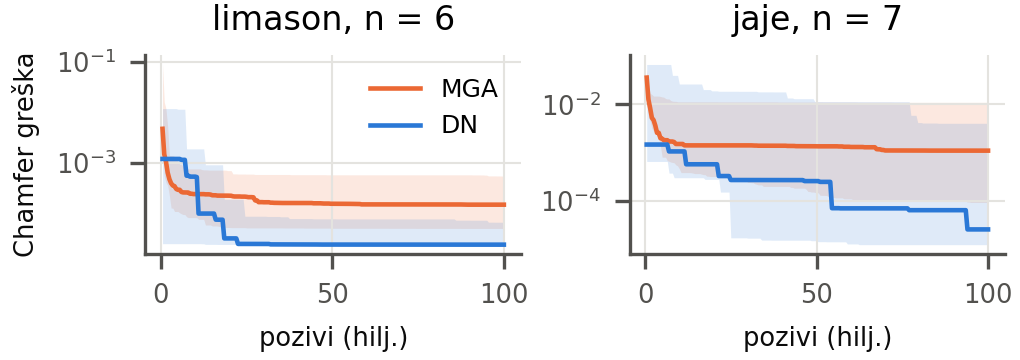
\includegraphics[width=\columnwidth]{slike/konvergencija_v5.png}
\caption{Najbolja greška u funkciji potrošenih poziva. Puna linija je
medijana preko seed-ova, pojas raspon od najboljeg do
najgoreg.\label{fig:konv}}
\end{figure}

Preko svih 115 parova, uz cenzurisanje na pun budžet tamo gde nikad ne
dostigne, DN dostiže konačnu grešku MGA na medijalno \textbf{24.5\%}
budžeta, a u 69\% parova na manje od polovine; u obrnutom smeru MGA
dostiže rezultat DN u samo 26 od 115 parova. Slika \ref{fig:konv}
pokazuje i oblik: DN napreduje stepenasto, skokom kad se pojavi
topologija čiju geometriju CMA-ES ume da odvede niže, dok MGA brzo pada
u prvih nekoliko hiljada poziva, a zatim sporo.

Medijana najmanjeg ugla prenosa je \(10.5^\circ\) za MGA i
\(10.8^\circ\) za DN, medijana glomaznosti 4.50 naspram 4.25, a prekida
putanje nema ni u jednom od 230 pokretanja: prednost u grešci nije
kupljena gorom izvodljivošću. Obe granice su aktivne --- dve trećine
rešenja ima ugao prenosa između \(10^\circ\) i \(15^\circ\), a polovina
glomaznost iznad 4.5. Pri fiksnom \(n\) DN ostvaruje manju grešku sa
manje radnih čvorova (5--6 naspram 6--7). Ali dve krive na kojima DN
nema jasnu prednost --- Kasinijev oval i superelipsa --- jedine su na
kojima nijedno od 46 pokretanja nije sišlo ispod \(4\cdot10^{-4}\): pri
datom \(n\) oba metoda stižu do istog poda, koji zavisi od \(n\) (na
superelipsi \(3.5\cdot10^{-3}\) pri \(n=6\), \(2.0\cdot10^{-3}\) pri
\(n=8\)). Taj pod daje i merilo veličine efekta: ceo dodatni čvor vredi
1.75×, pa je 0.62× po tom merilu krupan pomak. Tu se vidi vrednost
proširenja: u E2 DN sam raste do 9 radnih čvorova i stiže do
\(2.1\cdot10^{-3}\), dok MGA ostaje na 5.5 radnih čvorova i
\(3.6\cdot10^{-3}\) --- prednost nije bolji optimum pri istom \(n\),
nego bolji izbor veličine mehanizma.

\hypertarget{diskusija}{%
\section{Diskusija}\label{diskusija}}

Ong i sar. \citep{igbd} razlikuju četiri tipa uticaja kategoričkog dela
na kontinualni: maskiranje aktivnih komponenti (I), pomeranje optimuma
(II), oboje (III) i promenu metrike, tj. sprege među komponentama \(x\)
(IV). Skelet ovde određuje predačko stablo, dakle koje komponente \(x\)
utiču na putanju --- pri \(n=8\) rade svih osam čvorova u samo 25.5\%
generacija --- što je tip I po konstrukciji; oni navode da tip I traži
poseban tretman u donjem nivou, a ovde je to izostavljanje mrtvih
dimenzija. Promena oslonca ili znaka menja značenje svake komponente
nizvodnih čvorova --- tip II, dakle najmanje tip III.

Za tip IV Hesijan funkcije cilja po \(x\) meren je konačnim razlikama u
prijavljenim rešenjima matrice sa fiksnim \(n = 8\), dakle na istim
pokretanjima iz kojih dolaze rezultati; od 60 pokretanja 43 su
upotrebljiva, a kod ostalih stencil izlazi iz izvodljivog. Udeo energije
van dijagonale je 0.43--1.00, medijana 0.80: pejzaž je svuda jako
nerazdvojiv, što je nezavisan argument za unutrašnji metod sa punom
kovarijansom. Najveća sopstvena vrednost varira unutar iste krive i pri
istom broju aktivnih dimenzija, od 3.8× na elipsi do 71.8× na jajetu,
dakle skelet menja i oblik pejzaža. Kako skeleti nisu birani nego
zatečeni iz pretrage, tvrdnja o tipu IV ostaje potkrepljena, a ne
dokazana.

Poređenje menja dve stvari istovremeno: podelu pretrage na nivoe i izbor
unutrašnjeg optimizatora, pa doprinos svake od njih ostaje neizmeren.
Monolitna kontrola sa punom kovarijansom nije izvodljiva, jer u
monolitnom zapisu vektor geometrije menja značenje pri svakoj topološkoj
mutaciji --- isti broj u \(\rho\) opisuje drugu polugu, a pri dodavanju
čvora menja se i dimenzija --- dok učenje kovarijanse pretpostavlja
koordinate stalnog značenja. Dva metoda razdvajaju ono što ovo poređenje
spaja: CatCMA izoluje doprinos podele, jer punu kovarijansu zadržava nad
zajedničkom raspodelom, a IGBD izoluje oblik spoljašnjeg nivoa. Za
CatCMA argument predviđa slab rezultat baš ovde, jer proizvod-raspodela
pretpostavlja nezavisnost koju izmerena van-dijagonalna energija od 0.80
ne podržava.

Prednost se pojavljuje pod tri okolnosti kojih u njihovim
test-funkcijama nema: višeopcione kategoričke promenljive (do 21
opcije), neizvodljivost sa platoom kazne, i budžet od \(10^5\) poziva
naspram \(2\cdot10^4 d_c d_x\) koliko propisuje njihov protokol (za
\(n=8\) 28 puta manje).

Mera je uzeta nad šest seed-ova po ćeliji (pet za \(n=7\)), naspram
dvadeset u referentnom radu, i nad jednom klasom ciljnih krivih. U E2
koordinatna mutacija monolitnog metoda pogađa i čvorove van predačkog
stabla (medijalno 8.5 čvorova naspram 5 radnih), dok ih dvonivovski
metod izostavlja iz vektora; ta asimetrija ide u korist dvonivovskog
metoda i verovatno precenjuje njegovu prednost u E2, dok E1, gde mrtvog
tereta gotovo da nema, njome nije zahvaćen. Najzad, redukovani spektar
Hesijana ima medijalno tri negativne sopstvene vrednosti, dakle
prijavljeno najbolje rešenje nije strogi lokalni minimum: oba metoda
staju pre nego što je unutrašnji problem rešen do kraja.

\hypertarget{zakljuux10dak}{%
\section{Zaključak}\label{zakljuux10dak}}

Sinteza pantografskih mehanizama, zapisana kao sekvenca sklapanja, pri
fiksnom broju čvorova je tačna instanca mešovitog problema
\(\min f(c,x)\) iz rada Ong, Shirakawa i Akimoto. Na tom problemu
dvonivovski metod pri istom budžetu daje nižu grešku od monolitnog u 18
od 20 ćelija (medijana 0.62×), do rezultata monolitnog metoda dolazi na
četvrtini budžeta, bez gubitka fizičke izvodljivosti i sa manje radnih
čvorova. Prednost opstaje i pri promenljivom broju čvorova, gde okvir iz
reference ne važi, i tamo metod sam bira veličinu mehanizma. Prednost
nestaje tamo gde oba metoda pri datom broju čvorova stignu do granice
same familije mehanizama.

Dalji rad ide u tri pravca. Prvi je poređenje sa CatCMA i IGBD, jer se
tek njima razdvaja koliko prednosti dolazi od podele na nivoe, a koliko
od izbora unutrašnjeg optimizatora. Drugi je ciljna kriva dobijena iz
poznatog mehanizma, kod koje je najmanja moguća greška nula po
konstrukciji, pa se vidi koliko daleko od optimuma metodi staju. Treći
je sistematsko variranje skeleta pri fiksnom broju čvorova, čime bi
tvrdnja o tipu IV prešla iz potkrepljene u dokazanu.

Pri izradi programa, obradi rezultata i pisanju teksta korišćen je
asistent zasnovan na velikom jezičkom modelu (Claude, Anthropic); svako
merenje i zaključak autor je proverio, a kôd i logovi su objavljeni da
provera bude moguća i sa strane.

Kôd, logovi svih pokretanja i tačne komande nalaze se na
\texttt{github.com/najkela/generisanje-pantografskih-sistema}, oznaka
\texttt{ieeestec-2026}.

  \scriptsize\bibliography{bib.bib}

\end{document}
